\documentclass[a4paper]{article}
\usepackage{svn-multi}
% Version control information:
\svnidlong
{$HeadURL: https://practicas-spss.googlecode.com/svn/trunk/teorema_central_limite/teorema_central_limite.tex $}
{$LastChangedDate: 2010-09-27 16:37:11 +0200 (lun, 27 sep 2010) $}
{$LastChangedRevision: 3 $}
{$LastChangedBy: asalber $}
\svnid{$Id: teorema_central_limite.tex 3 2010-09-27 14:37:11Z asalber $}
\pdfinfo{/CreationDate (D:\svnpdfdate)}
\svnRegisterAuthor{alf}{Alfredo Sánchez Alberca}

\usepackage[spanish]{babel}
\usepackage[utf8x]{inputenc}
\usepackage{amsmath}
\usepackage{macros}
\usepackage[dvips]{graphicx}
\usepackage{enumitem}
\usepackage{subfigure}
\usepackage[small,bf]{caption2}
\usepackage[top=3cm, bottom=3cm, left=2.54cm, right=2.54cm]{geometry}
\usepackage{fancyhdr}
\pagestyle{fancy}

\lhead{\textsc{Universidad San Pablo CEU}} \rhead{\textsl{\textsf{Departamento de Métodos Cuantitativos}}}
\renewcommand{\headrulewidth}{0pt}
\renewcommand{\floatpagefraction}{.8}
\renewcommand{\textfraction}{.1}
\setcaptionwidth{\textwidth} \addtolength{\captionwidth}{-40pt}
\captionstyle{indent} \setlength\captionindent{\parindent}

\makeatletter
\let\savees@listquot\es@listquot
\def\es@listquot{\protect\savees@listquot}
\makeatletter

\begin{document}
\sloppy

\practica{Práctica de Estadística con Statgraphics}{Teorema
Central del Límite}

\bigskip
\section*{Fundamentos teóricos}
\subsection*{Importancia de la Distribución Normal}
La distribución normal resulta especialmente importante porque
aproxima lo observado en muchos procesos de medición. Por ejemplo,
las medidas físicas del cuerpo humano en una población, las
características psíquicas medidas por un test de inteligencia o
personalidad, la nota de un examen de Bioestadística, las medidas
de calidad en muchos procesos industriales, el tiempo de
recuperación de una determinada lesión, o la mejoría experimentada
en ciertos niveles biológicos después del tratamiento con un
fármaco.

\subsection*{El Teorema Central del Límite}
La justificación de la frecuente aparición de la distribución
normal proviene del \emph{Teorema Central del Límite}, que
establece que cuando los resultados de un experimento son debidos
a un conjunto muy grande de causas independientes que actúan
sumando sus efectos, siendo cada efecto individual de poca
importancia respecto al conjunto, es esperable que los resultados
sigan una distribución normal.

En términos más matemáticos este teorema establece que si
$X_{1},...,X_{n}$ son variables aleatorias independientes con
distribución cualquiera (no necesariamente la misma), media
$\mu_{i}$ y varianza $\sigma_{i}^{2}$, y construimos la variable
suma:

\[
Y = X_1  + ... + X_n
\]
entonces, cuando $n$ crece, la variable $Y$ sigue una distribución
normal cuya media es la suma de medias y cuya varianza es la suma
de varianzas:

\[
Y \sim N\left( {\Sigma \mu _i ,\sqrt {\Sigma \sigma _i ^2 } }
\right)
\]

El valor de $n$ variará según las variables aleatorias de las que
se trate. Como valor orientativo suele darse $n \geq 30$. Sin
embargo, si las variables de partida son continuas, simétricas y
están idénticamente distribuidas, la aproximación se consigue para
valores de $n$ mucho más pequeños. Para distribuciones discretas
puede ser necesario incluso un valor de $n$ mayor o igual que 30
para tener una buena aproximación.

\begin{figure}[h!]
\begin{center}
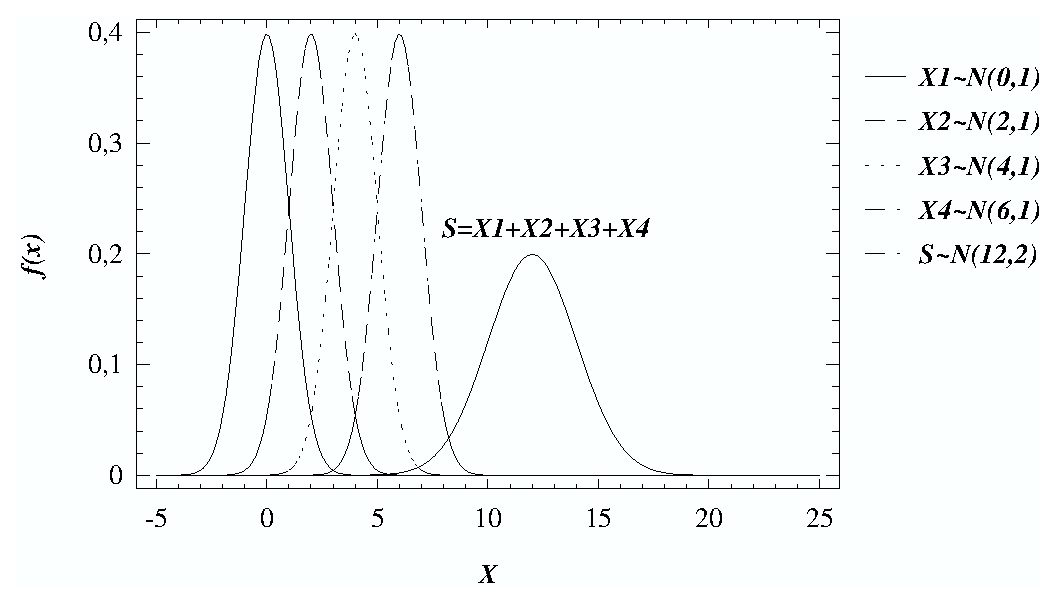
\includegraphics[scale=0.7]{grafica1.eps}
\caption{El Torema Central del Límite partiendo de 4
distribuciones normales.}
\end{center}
\end{figure}



\subsection*{Aplicaciones del Teorema Central del Límite}

Si aplicamos el Teorema Central del Límite a la suma de $n$
variables independientes idénticamente distribuidas, y por lo
tanto con igual media, $\mu$, y desviación típica, $\sigma$, la
variable suma resultante se distribuirá según una normal de media
$n \mu$ y desviación típica $\sigma \sqrt n$:

\[
Y \sim N\left( n \mu , \sigma \sqrt n \right)
\]

\subsubsection*{Distribución para la Media Muestral}

Si tenemos en cuenta que la \emph{variable media muestral} resulta
como suma de $n$ variables idénticamente distribuidas:

\[
\overline X  = \frac{1}{n}\sum\limits_{i = 1}^n {X_i }
\]
y aplicando propiedades de la media y la varianza, junto con el
Teorema Central del Límite, puede demostrarse fácilmente que la
media muestral sigue una distribución normal de media $\mu$ y
desviación típica $\sigma / \sqrt{n}$ :

\[
\overline X \sim N\left( {\frac{{n\mu }}{n},\frac{{\sigma \sqrt n
}}{n}} \right) = N\left( {\mu ,\frac{\sigma }{{\sqrt n }}} \right)
\]

Resultado este último muy importante y especialmente utilizado en
Inferencia Estadística.

\begin{figure}[h!]
\begin{center}
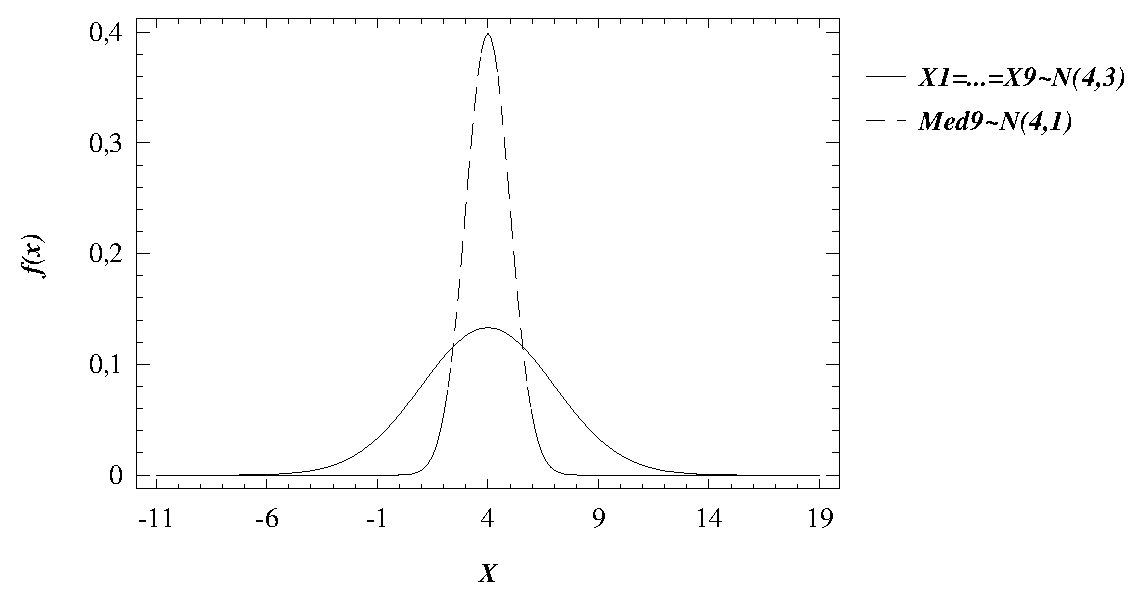
\includegraphics[scale=0.7]{grafica2.eps}
\caption{Distribución de la Media Muestral de 9 variables normales
de media 4 y desviación típica 3.}
\end{center}
\end{figure}


\subsubsection*{Aproximación de la Binomial mediante una Normal}

Si tenemos en cuenta que la variable binomial se obtiene como suma
de $n$ variables de Bernouilli, idénticamente distribuidas, cada
una de ellas con valores 0 ó 1 (éxito o fracaso), de media $p$
(probabilidad de éxito) y desviación típica $\sqrt{p(1-p)}$, y si
suponemos que $n\geq 30$, $np>5$ y $n(1-p)>5$ (estas dos últimas
condiciones para garantizar la simetría de la distribución),
entonces podemos aplicar el Teorema Central del Límite y afirmar
que la variable Binomial se podrá aproximar mediante una normal de
media $np$ y desviación típica $\sqrt{np(1-p)}$.

\[
X\sim N\left( {np,\sqrt {np\left( {1 - p} \right)} } \right)
\]

El anterior resultado se conoce como \emph{Teorema de De Moivre} y
también se aplica muy frecuentemente en Inferencia Estadística.


\section*{Ejercicios Prácticos}
\begin{enumerate}[leftmargin=*]

\item Para comprobar el cumplimiento del Teorema Central de Límite
partiendo de 4 variables con distribución uniforme entre $[0,10]$,
se pide:

\begin {enumerate}

\item Crear la variable \textsf{Unif1} que contenga una muestra de 1000 valores
generados aleatoriamente a partir de una variable aleatoria uniforme entre 0 y 10. 
\begin{indicacion}{
\begin{enumerate}
\item Seleccionar el menú \texttt{Gráficos->Distribuciones de Probabilidad}.
\item Seleccionar \texttt{Uniforme} en el cuadro de diálogo que aparece.
\item Hacer click con el botón derecho del ratón sobre la ventana de resultados obtenida y seleccionar \texttt{Opciones de Análisis}.
\item Introducir el valor del límite inferior de la Uniforme en el campo \texttt{Límite Inferior} y el del límite superior en el campo \texttt{Límite Superior}. 
\item Hacer click en el botón \texttt{Opciones Tabulares} y activar la casilla \texttt{Números Aleatorios}.
\item Hacer click con el botón derecho del ratón sobre la ventana de resultados obtenidos y seleccionar \texttt{Opciones de Ventana}.
\item Introducir el tamaño de la muestra en el campo \texttt{Tamaño}.
\item Hacer click en el botón \texttt{Guardar Resultados}.
\item En el cuadro de diálogo que aparece, activar la casilla \texttt{Números Aleatorios para Dist.1} y escribir el nombre de la variable a generar en el campo \texttt{Variable Destino}.
\end{enumerate}}
\end{indicacion}

\item Comprobar que los valores de la variable \textsf{Unif1} se distribuyen
uniformemente entre 0 y 10. Para ello, dibujar el histograma de
dicha variable haciendo 10 clases y comprobar que la
frecuencia de cada clase es aproximadamente 100.
\begin{indicacion}{
\begin{enumerate}
\item Seleccionar el menú \texttt{Descripción->Datos Numéricos->Análisis Unidimensional}.
\item Seleccionar la variable \textsf{Unif1} en el campo \texttt{Datos} del cuadro de diálogo.
\item Hacer click en el botón \texttt{Opciones Gráficas} y activar la casilla \texttt{Histograma}.
\item Hacer click con el botón derecho del ratón sobre el histograma obtenido y seleccionar \texttt{Opciones de Ventana}.
\item Introducir el número de clases y los límites superior e inferior de la partición en los campos correspondientes.
\end{enumerate}}
\end{indicacion}

\item Calcular la media y la desviación típica de la variable Unif1 y comprobar si se parecen a media y desviación típica de una variable aleatoria uniforme [0,10]. (recordar que la media de una distribución uniforme [a,b] es
$(b+a)/2$ y su desviación típica $(b-a)/\sqrt{12})$).
\begin{indicacion}{
\begin{enumerate}
\item En la misma ventana del apartado anterior hacer click en el botón \texttt{Opciones Tabulares} y activar la casilla \texttt{Resumen Estadístico}.
\item Hacer click con el botón derecho del ratón sobre los resultados obtenidos y seleccionar \texttt{Opciones de Ventana}.
\item Activar las casillas correspondientes a los estadísticos que se piden.
\end{enumerate}}
\end{indicacion}

\item Crear tres variables más \textsf{Unif2}, \textsf{Unif3} y \textsf{Unif4} que contengan otras 3 muestras de 1000 valores generados aleatoriamente a partir de una variable aleatoria uniforme entre 0 y 10. 

\item Crear la variable \textsf{Suma} que contenga la suma de los valores de las muestras generadas previamente.
\begin{indicacion}{
\begin{enumerate}
\item Con la variable \textsf{Suma} seleccionada en el editor de datos, seleccionar el menú \texttt{Edición->Generar Datos}.
\item En el editor de fórmulas, escribir la expresión que da origen a la nueva variable.
\end{enumerate}}
\end{indicacion}

\item Dibujar el histograma que la variable \textsf{Suma}. ¿Qué forma presenta el histograma? ¿A qué distribución se parece?
\begin{indicacion}{
\begin{enumerate}
\item Seleccionar el menú \texttt{Descripción->Datos Numéricos->Análisis Unidimensional}.
\item Seleccionar la variable \textsf{Suma} en el campo \texttt{Datos} del cuadro de diálogo.
\item Hacer click en el botón \texttt{Opciones Gráficas} y activar la casilla \texttt{Histograma}.
\end{enumerate}}
\end{indicacion}

\item Calcular la media, la desviación típica, el coeficiente de asimetría y el coeficiente de curtosis de la variable \textsf{Suma}. Si se cumple el Teorema
Central del Límite, ¿cuáles deberían ser los valores estos estadísticos? ¿Hay grandes diferencias entre los valores que predice dicho teorema y los realmente obtenidos?
\begin{indicacion}{
\begin{enumerate}
\item En la misma ventana del apartado anterior hacer click en el botón \texttt{Opciones Tabulares} y activar la casilla \texttt{Resumen Estadístico}.
\item Hacer click con el botón derecho del ratón sobre los resultados obtenidos y seleccionar \texttt{Opciones de Ventana}.
\item Activar las casillas correspondientes a los estadísticos que se piden.
\end{enumerate}}
\end{indicacion}

\item Crear la variable \textsf{Media} que contenga la media de los valores de las muestras generadas previamente.

\item Dibujar el histograma que la variable \textsf{Media}. ¿Qué forma presenta el histograma? ¿A qué distribución se parece?
\begin{indicacion}{
\begin{enumerate}
\item Seleccionar el menú \texttt{Descripción->Datos Numéricos->Análisis Unidimensional}.
\item Seleccionar la variable \textsf{Media} en el campo \texttt{Datos} del cuadro de diálogo.
\item Hacer click en el botón \texttt{Opciones Gráficas} y activar la casilla \texttt{Histograma}.
\end{enumerate}}
\end{indicacion}

\item Calcular la media, la desviación típica, el coeficiente de asimetría y el coeficiente de curtosis de la variable \textsf{Media}. Comparar la media y desviación típica obtenidas con las de las variables de partida.
¿Se cumple el Teorema Central del Límite aplicado a la distribución de la media muestral?
\begin{indicacion}{
\begin{enumerate}
\item En la misma ventana del apartado anterior hacer click en el botón \texttt{Opciones Tabulares} y activar la casilla \texttt{Resumen Estadístico}.
\item Hacer click con el botón derecho del ratón sobre los resultados obtenidos y seleccionar \texttt{Opciones de Ventana}.
\item Activar las casillas correspondientes a los estadísticos que se piden.
\end{enumerate}}
\end{indicacion}
\end{enumerate}

\item Para comprobar que la aproximación de la binomial mediante una normal se deduce del Teorema Central del Límite, repetir los apartados del ejercicio anterior generando las muestras a partir de una distribución binomial de parámetros $n=100$ y $p=0.4$.

\end{enumerate}

\section*{Problemas}
\begin{enumerate}[leftmargin=*]

\item Crear 4 variables aleatorias que contengan muestras de 1000 valores generadas aleatoriamente a partir de distribuciones $N(10\,,\,5)$, $P(10)$, $B(20\,,\,0.5)$ y $U(5\,,\,15)$ respectivamente y repetir los pasos de los ejercicios anteriores para ver si se cumple el Teorema Central del Límite.

\end{enumerate}
\end{document}
